\begin{quoting}
Isolation is easy, sharing is hard.
\todo[inline]{find original source or use Casey's name}
\end{quoting}


The notion of access control (AC) and application/process isolation is one of the oldest in the history of the information security with first pioneering works being done back in 80-ies. Initially the main goal of AC methods was to isolate different system's users with different level of access to the system assets, but as computers and other IT devices started to become more and more single-user purpose, the focus has shifted towards isolation of system processes and applications. This trend was especially noticeable in various mobile platform security architectures, when users got the ability to install third-party software on their mobile devices because it required a stricter isolation between system's core platform and services (trusted set of entities) and user installable services and applications (untrusted and potentially malicious).

A typical AC system can be viewed as a collection of one or more AC reference monitors that are consulted for AC decisions whenever any system access (such as operation on a filesystem object) is performed. The AC decision is done based on the AC policy for that AC reference monitor and defines if the access should be allowed or not. The AC policy is written in a form of AC rules that are defined in terms of \textit{subjects} (active entity performing the access), \textit{objects} (passive entity that is being accessed) and \textit{access types} (what type of access is being attempted, such as read, write etc.). Subject and objects are also typically grouped into a set of \textit{access control domains} using some identification or labeling scheme, allowing policy writers to arrange related and interconnected OS components into logical blocks. Typically most of the AC systems employ the principle that by default any access is denied unless explicitly allowed by AC policy rules or both subject and object are belonging to the same access control domain.
 
Over the decades the topic of process and application isolation was a focus for tremendous amount of academia and industrial research works with many systems and mechanisms proposed to address the problems arising when designing and implementing AC systems. On a high level these problems can be arranged into the following categories that are all interconnected and affecting each other: 

\begin{itemize}
	\item \textbf{Granularity.} One can design and deploy AC mechanisms with very different granularity levels following the principle of least privilege. On one side is placing each individual process or thread into its own access control domain, and on the other side only creation of high-level access control domains that would isolate the trusted part of the system from user-installable and less trusted applications. It is clear that a fine-grained AC policy allows creating a more precise set of AC rules for a given AC object, however it usually directly negatively impacts other factors like manageability and performance making policy writers and designers to search for some intermediate balance.    
	\item \textbf{Manageability.} Most modern mobile and embedded OSes change at a high pace: new system services and APIs being introduced with each release, existing services might be fully redesigned, new use cases might be introduced etc. Same applies for the system's AC policy: it must adapt and change with the system to make sure it not only correctly reflects the current state of the system, but also correctly isolates and protects its entities. In addition one needs to take into account how OS is being developed. For example if OS changes are done in distributed fashion by different independent set of development teams, the policy needs to be modular enough to allow changes to be performed relatively independently and in parallel. One just cannot assume that there is a single person that can manage all policy changes centrally.  
	\item \textbf{Performance.} Typically an access control system is integral part of an OS and for every system access, an access control decision needs to be made based on available parameters. This makes an AC mechanism a very run-time performance sensitive component and care needs to be taken to make the overhead acceptable for system use. 
\end{itemize}

Part of this thesis investigates how the modern AC mechanisms attempt to find a balance in the above categories, what are the concrete problems that they are facing in a struggle to find this balance, as well as to understand what tools or techniques can be helpful in practice to solve these problems. For this purpose the thesis selects one of the most popular mobile operating system, Android and its mandatory AC mechanism, SEAndroid for a detailed evaluation as the most used mandatory AC mechanism on mobile and embedded Linux-based OSes. Another focus area of this thesis is an attempt to look into alternative ways how process and application isolation can be done using various OS-level virtualization  techniques (aka application or system containers) that during couple of last years became a fashionable alternative to traditional AC mechanisms. The main research question that this thesis attempts to answer with regards to the OS-level virtualization is whenever this technique can provide a similar level of security that traditional mandatory AC mechanisms. 


\section{Mandatory access control on modern systems: SEAndroid}

Over the past decades, Android has become one of the most common OSes for mobile devices. As the amount of devices running Android has been increasing, so was the amount of malware targeting this operating system. Back in 2011 it became clear that the discretionary Android permission access control model is not able to provide the required level of security and the work started on adapting the well-known desktop mandatory access control mechanism, SELinux, for the purpose of Android OS. The resulting mechanism, SEAndroid, was largely based on SELinux, but contained some adjustments and additions required for the supporting some of Android-specific mechanisms, such as Binder Inter Process Communication (IPC). The biggest change was the SEAndroid reference policy, which was written from scratch and due to significant differences in the Android and desktop userspace layer, as well as a desire to have a small and compact policy. The initial policy and enforcement points were added to the Android 4.3 release back in 2012, but it wasn't until Android 5.0 Lollipop release when SEAndroid was required to be enabled on all devices in the system-wide enforcing mode, which forced OEMs to start working on SEAndroid policies. 

Traditionally the Android ecosystem works in a way that Google delivers the reference code for the Android OS in a form of open source AOSP project, which is taken by different Android OEMs and customized at various levels starting from HW adaption, new OEM-specific drivers and system services, and ending up some user facing applications. The reference SEAndroid policy, provided by the AOSP project, does not obviously cover these additions and customizations, and therefore OEMs need to adjust the provided SEAndroid policy not only to get to a desired level of mandatory access control enforcement, but also merely to make their customized Android OS work correctly.

The publication II of this thesis starts by examining 8 different SEAndroid policies from various Android OEMs that was created for Android 5.0 release and provides extensive characteristics of these policies in terms of OEM-performed changes, policy size and complexity and etc. Table 1 from publication II shows that all OEMs extensively modify the reference policy resulting in overall policy size growth, as well as all other policy attributes and access control rules. Next the publication II manually analyzes the characteristics of each of these 8 policies and builds a set of typical pitfalls that all OEMs seems to make when performing their policy additions. These include overuse of default types, where many OEMs leave SEAndroid default labels\footnote{if an object is not given an explicit label by the SEAndroid policy, it is assigned one of the default labels, such as \setype{unlabeled}, \setype{device}, \setype{default\_prop} etc.} for their newly added system objects, which typically leads to aggregation of big amount of non-related objects under a single default label and consequently leads to the violation of the principle of least privilege since many different domains might need to have legitimate access to the objects under default labels. Another typical pitfall pattern is aggregation of OEM-created applications under the reference policy predefined application domains, such as \setype{platform\_app} or \setype{system\_app} instead of creation of smaller, OEM-specific application domains. This leads to the enormous grow of such default domains (for example one OEM policy had 900 allow rules associated with \setype{system\_app} domain vs. 46 in the AOSP reference policy) and inability to prevent privilege escalation between different OEM applications placed in these domains. Other OEMs pitfalls include seemingly useless or forgotten rules, as well as rules that are dangerous for the overall security of the system (such as granting access to rather sensitive parts of the system to the untrusted domains), which indicate that OEMs struggled to deliver the comprehensive and secure SEAndroid policies on their devices. 

\begin{figure}[t]
	\centering
		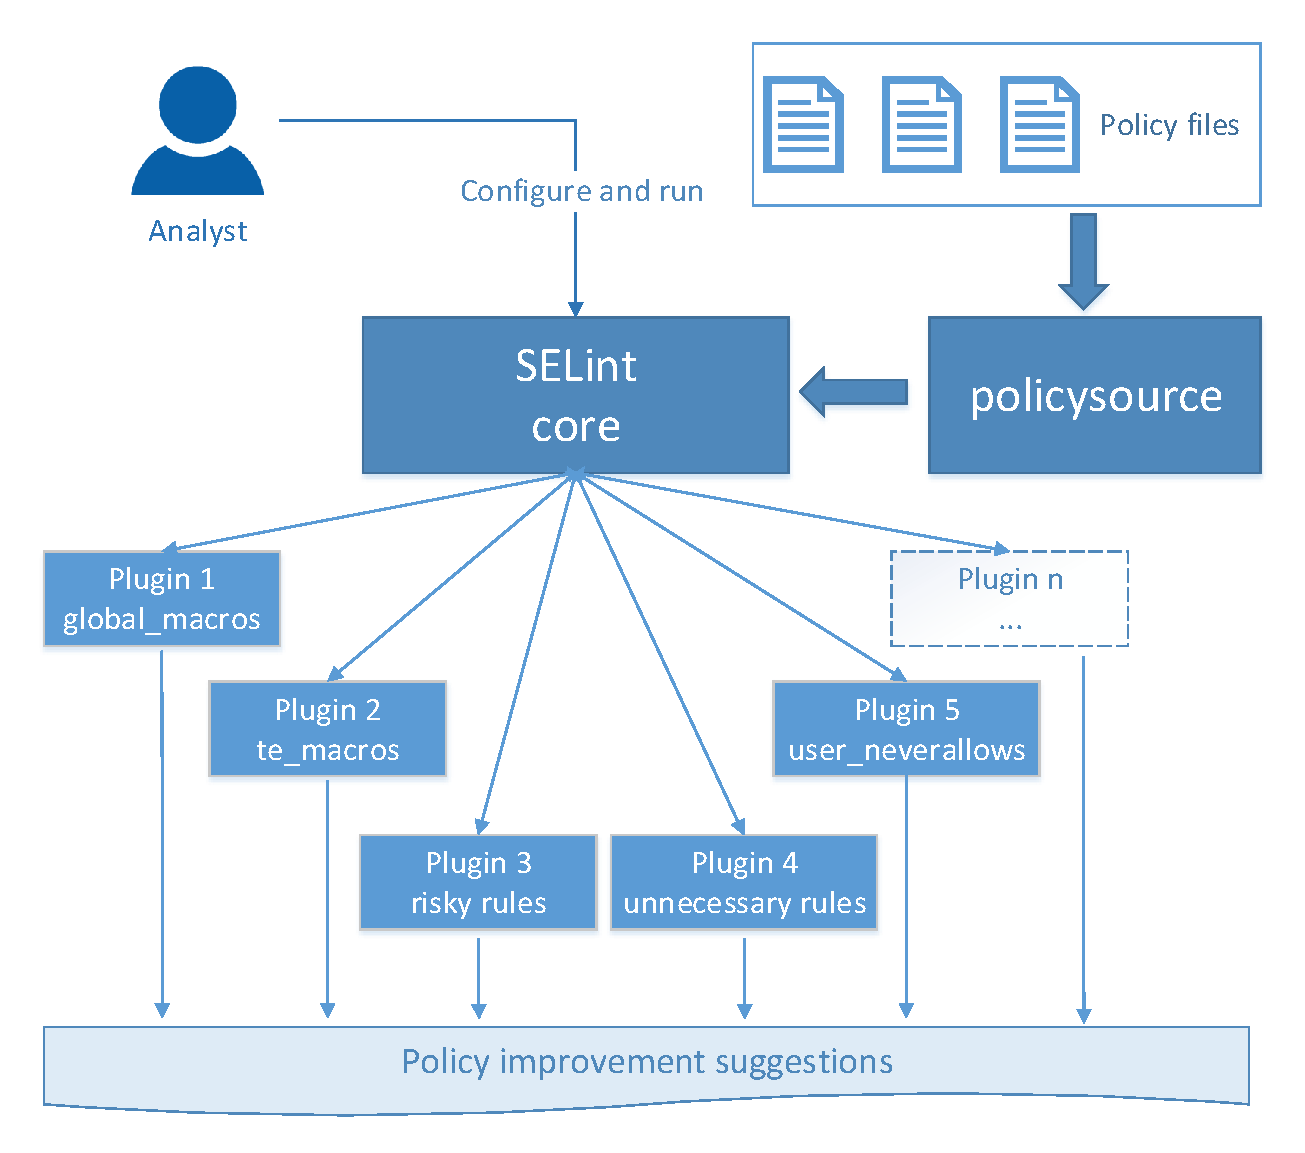
\includegraphics[width=0.80\textwidth]{figures/selint-archi.pdf}
	\caption{The architecture of SELint (From Publication III)}
	\label{fig:selint}
\end{figure}

\todo[inline]{Remember to either get the copyright permission or modify the figure}   

As a result of above study the publication II proposes a set of tools that should help both OEMs and security researchers to develop better SEAndroid policies without the above-mentioned pitfalls, including various policy analyzing and virtualization tools. It also implements one of such tools, a live SEAndroid policy analyzer (SEAL), that allows performing different policy queries not only based on the actual policy loaded on the devices, but also also a run-time device state, i.e. running processes and services, filesystem labeling etc. SEAL allows to get a fast answer on various questions that a SEAndroid policy writer or analyzer might have, such as "What files can a given running process access on a device?" or "What processes can access a given object?". This significantly simplifies the debugging, troubleshooting and studying a given SEAndroid policy and gives a fast way to discover the inconsistencies. 

The publication III presents the design and implementation of a more comprehensive SEAndroid tool, SELint, that is designed for an overall improvement of SEAndroid policy development. It operates on SEAndroid policy sources and allows smooth integration into the OEM policy development workflow. The architecture of SELint is shown in Figure~\ref{fig:selint}. It is composed from a SELint core, responsible for the heavy processing of input SEAndroid policy files, and an initial set of SELint plugins that operate on a policy representation provided by the core and able to do the policy analysis. The set of plugins is designed to be extensible and adapt to the needs of different OEMs or security researchers. The initial set of plugins includes 5 distinct ones: two plugins (\setype{global\_macros} and \setype{te\_macros}) verifying correctness of usage different types of SEAndroid policy macros, a \setype{user\_neverallows} plugin that allows a OEM-specific verification of additional neverallow rules, a \setype{unnecessary\_rules} plugin that attempts to detect various ineffective rules\footnote{some rules in SEAndroid policy are only effective in combination with others, such as domain transition rules when a process wants to transition its domain to a different one upon opening a certain type of object} or rules used for debug purposes, and finally a \setype{risky\_rules} plugin that can be used to categorize SEAndroid access control domains into set of related ones (untrusted, security-sensitive, core tcb etc.) and display various risk and trust relationships between them in a given policy. For example, it is possible to highlight the access control rules where access to a security-sensitive object is given to a subject belonging to an untrusted domain.


\section{Application and process isolation using OS-level virtualization}

While traditional access control mechanisms and systems aiming for application and process isolation has existed for decades, recent years have seen a raise of an alternative approach, OS-level virtualization techniques, more commonly known as "`containers"'. While originally developed purely to support various virtualization-based use cases, such as server consolidation or application and resource state management, they later on turned into various security-driven use cases, such as application isolation and Bring Your Own Device (BYOD) scenario\footnote{a single physical device is used for both business and personal purposes that requires a strict isolation between these two environments and limited sharing}.  

In contrary to the traditional virtualization solutions, like well-known Xen hypervisor or Linux Kernel Virtual Machine (KVM), an OS-level virtualization virtualizes the OS kernel resources available to userspace, as opposite to the actual physical HW resources, and therefore allows processes to share the same host OS kernel. This greatly reduces the performance overhead incurred by the OS-level virtualization and consequently it became possible to use this technology for an efficient isolation of stand-alone applications or their sets.

Parallel to their popularity, there is a constant debate about the security level that such virtualization provides in practice, as well as an attempt to find the gaps in the current implementations. The publication IV of this thesis identifies the security requirements and generic model for a typical OS-level virtualization setup, and then compares a selection of available (both present and historical) solutions with regards to this model. 


\begin{figure}[t]
\centering
\begin{subfigure}{.5\textwidth}
  \centering
  \includegraphics[width=0.8\linewidth]{figures/os-virtualization-sys-model.png}
  \caption{System model}
  \label{fig:osv-1}
\end{subfigure}%
\begin{subfigure}{.5\textwidth}
  \centering
  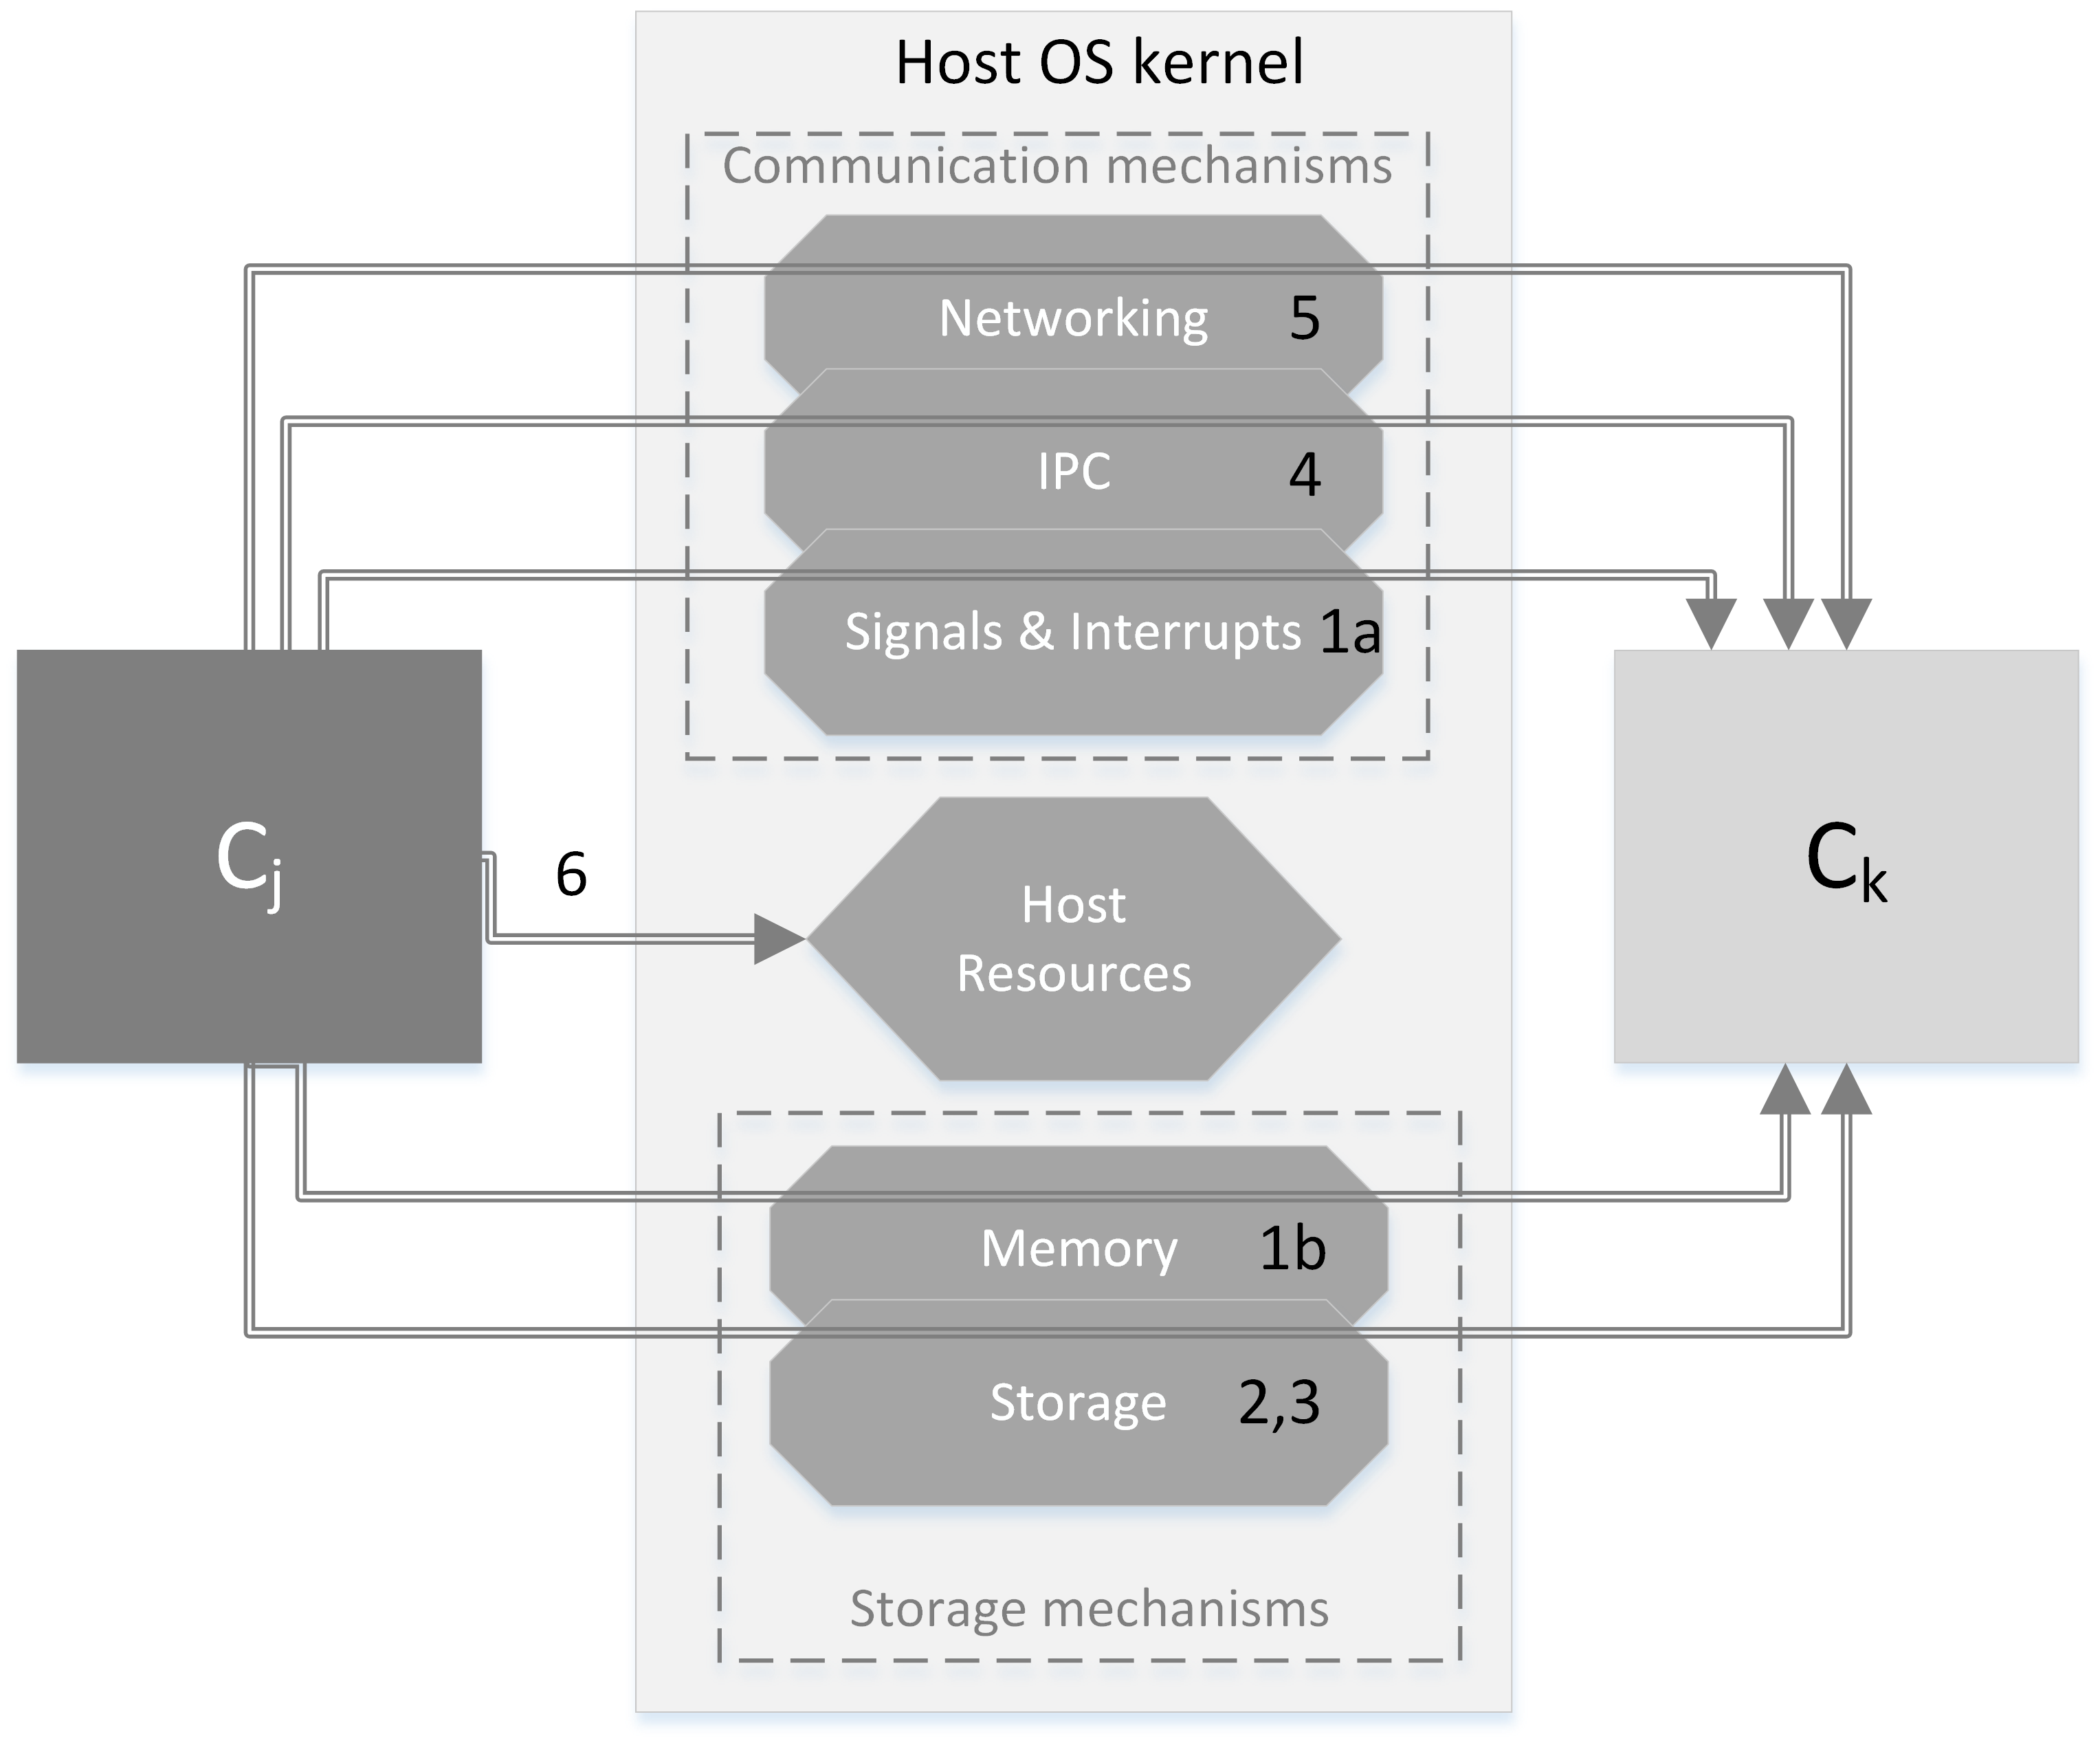
\includegraphics[width=1\linewidth]{figures/OS-virtualization-attacker-model.png}
  \caption{Attacker model}
  \label{fig:osv-2}
\end{subfigure}
\caption{OS-level virtualization}
\label{fig:os-virtualization}
\end{figure}

The system and attackers model for OS-level virtualization are shown in Figure~\ref{fig:os-virtualization}. The set of containers C1..CN are running on top of shared host OS kernel and userspace layers. The latter one can be either minimal layer only responsible for doing the setup of containers or a full fledged host OS userspace layer. The attacker model assumes that an attacker has a full control over a certain subset of containers and attempts to attack either another subset of legitimate containers running on the same host or host OS itself with either of these three goals: privilege escalation, legitimate container or host compromise or denial-of-service. Each of this can be achieved by one of the attack groups that can be roughly classified based on typical interfaces available to a UNIX-compliant OS (1-6 in Figure~\ref{fig:osv-2}). These attack groups are then converted into security requirements that each OS-level virtualization solution must fulfill in order to provide strong isolation: separation of processes, filesystem isolation, device isolation, IPC isolation, network isolation and resource management.   

The publication IV analyzes 6 OS-level virtualization solutions against the above security requirements and outlines the differences in provided level of isolation. It also summaries the state of OS-level virtualization in the mainline Linux kernel, together with the identified gaps that were limiting the usage of this technology in the environments with strict security isolation requirements. However in the years after the publication IV was done many of these gaps has been either addressed by the mainline Linux kernel or have progressed towards a more robust solution:

\begin{itemize}
	\item Security namespaces. 
	\item Device namespaces.
	\item (Pseudo)random number generator devices. 
	\item Hotplug support. 
	\item Cgroups support. 
\end{itemize}

In addition a lot of work has been put into namespacing the rest of Linux kernel security subsystems, such as Integrity Measurement Architecture (IMA), Kernel Keyring etc.

\section{Discussion}

While the implementation of the OS-kernel virtualization in the mainline Linux kernel continues to evolve and improve, the classical mandatory access control schemes are still required to be jointly used in order to provide the highest possible level of isolation and minimize the security risks. Security architects must understand in details the limitations of OS-kernel virtualization in order to make well-grounded choices on a set of isolation mechanisms that their system is required in order to fulfill the security requirements for its use cases. The publication IV of this thesis presents a good model for such evaluation and comparison of available mechanisms, as well as guidance on identifying the missing isolation gaps. 

The SEAndroid MAC continues to be the main AC enforcement point of Android OS with all major OEMs now accustomed to the task of working with SEAndroid policies. The evaluation of initial SEAndroid policies done in publication II has been crossed referenced in the official Google SEAndroid documentation as a valuable insight into practical state of things. The SEAndroid tools proposed in publications II and III are being used by the Android community with numerous private forks done on the project code trees and bug reports filled by the users once in a while\footnote{https://github.com/seandroid-analytics}. The SELint tool fulfills the set of main functional R1 - R4 requirements defined in Section IV of Publication III by exhibiting an acceptable performance overhead, allowing its usage by ordinary users (after an initial expert configuration), being flexible and easy extensible. The detailed evaluation can be found in Section V of Publication III. 



